\documentclass{article}

\usepackage[final,nonatbib]{neurips_2019}

\usepackage[utf8]{inputenc} % allow utf-8 input
\usepackage[T1]{fontenc}    % use 8-bit T1 fonts
\usepackage{hyperref}       % hyperlinks
\usepackage{url}            % simple URL typesetting
\usepackage{booktabs}       % professional-quality tables
\usepackage{amsfonts}       % blackboard math symbols
\usepackage{nicefrac}       % compact symbols for 1/2, etc.
\usepackage{microtype}      % microtypography

\usepackage{amsmath}
\usepackage{amssymb}
\usepackage{mathtools, nccmath}
\usepackage[mathscr]{euscript}  % euler script font
\usepackage{cleveref}
\usepackage{enumitem}
\usepackage{algorithm}
\usepackage[noend]{algpseudocode}

\usepackage{listings}
\usepackage{xcolor}

\definecolor{codegreen}{rgb}{0,0.6,0}
\definecolor{codegray}{rgb}{0.5,0.5,0.5}
\definecolor{codepurple}{rgb}{0.58,0,0.82}
\definecolor{backcolour}{rgb}{0.95,0.95,0.92}

\lstdefinestyle{mystyle}{
    backgroundcolor=\color{backcolour},
    commentstyle=\color{codegreen},
    keywordstyle=\color{magenta},
    numberstyle=\tiny\color{codegray},
    stringstyle=\color{codepurple},
    basicstyle=\ttfamily\footnotesize,
    breakatwhitespace=false,
    breaklines=true,
    captionpos=b,
    keepspaces=true,
    numbers=left,
    numbersep=5pt,
    showspaces=false,
    showstringspaces=false,
    showtabs=false,
    tabsize=2
}

\lstset{style=mystyle}

\newtheorem{theorem}{Theorem}
\DeclareMathOperator{\Var}{Var}
\DeclareMathOperator{\modexp}{mod\_exp}
\DeclareMathOperator{\decryptiontime}{decryption\_time}
\DeclareMathOperator{\extrareduction}{extra\ reduction}

\title{Timing Attacks against RSA}

\author{%
  Lorenzo Palloni\\
  University of Florence\\
  \texttt{lorenzo.palloni@stud.unifi.it} \\
}

\begin{document}

\maketitle

%----------------------------------------------------------------------------------------
\section{Introduction}

Side-channel attacks exploit physical parameters such as execution time, supply current and electromagnetic emission to retrieve secrets from a system. A timing attack is a type of side-channel attack that, by measuring time differences in data-dependent operations of a cryptosystem, can expose its secret key. This report describes two major timing attacks against RSA, that is a public-key cryptosystem that is widespread in computer security applications.

In 1996, Kocher was the first to design a timing attack against cryptosystems based on modular exponentiation, such as RSA \cite{bib:kocher}. His work pushed enhancements of modular exponentiation implementations. If adopted, they make the original attack ineffective.

Almost ten years later, in 2005, Brumley and Boneh proved that timing attacks were practical on network servers based on OpenSSL\footnote{Throughout this report, we refer to OpenSSL version 0.9.7, unless otherwise specified.}, a commonly used library that implements RSA with several improvements \cite{bib:openssl}. In their experiments, they retrieved whole RSA private keys in time frames of approximately two hours, even through web servers with multiple network switches. Their work prompted OpenSSL developers, as well as other crypto libraries, to set up the defence technique "blinding" in RSA implementations by default.

%----------------------------------------------------------------------------------------



%----------------------------------------------------------------------------------------
\section{Technical background}\label{sec:technical}
The following sections cover some of the tools that will be useful to understand how the timing attacks work.

First, we introduce some notation while explaining the RSA cryptosystem, then we present the fast modular exponentiation algorithm, and how it can be optimized using Chinese Remainder, Sliding Windows, Montgomery multiplication, and Karatsuba's algorithm. These enhancements are all implemented in the version of OpenSSL on which Brumley and Boneh designed their attack.

\subsection{RSA}
Assume two agents - Alice and Bob - want to communicate each other and, in particular, Alice wants to send a message $m$ to Bob. However, they are using a public channel, and a third agent - Oscar - is able to read $m$ once sent. Alice and Bob can achieve confidentiality, if they agree on a secret, a key $k$, in advance. Then Alice can mask the plaintext $m$, using $k$, in an unintelligible ciphertext $c$ such that only Bob with $k$ can understand it.

In computer security, confidentiality can be attained using a cryptosystem, that is defined as a set of three components: a key generator, an encryption function and a decryption function.

RSA is a public-key cryptosystem that brings the surnames of Ron Rivest, Adi Shamir and Leonard Adleman who published the algorithm in 1977.
The key generation process of RSA can be described as follow:
\begin{enumerate}
  \item choose two prime numbers $p$, $q$, where $p \neq q$.
  \item compute the modulus $n = p \cdot q$.
  \item compute the Euler's function $\phi(n) = \phi(p) \cdot \phi(q) = (p - 1) \cdot (q - 1)$.
  \item choose an integer $e: 1 < e \leq \phi(n)$ and $\gcd(e, \phi(n)) = 1$.
  \item compute $d = e^{-1} \bmod \phi(n)$.
\end{enumerate}
The pair $\left< n, d\right>$ is the private key $K^-$, while $\left< n, e\right>$ is the public key $K^+$.

The encryption function $E_{K^+}: \mathcal{P} \rightarrow \mathcal{C}$ and the decryption function $D_{K^-}: \mathcal{C} \rightarrow \mathcal{P}$ are respectively defined as $E_{K^+}[m] := m^e \bmod n$ and $D_{K^-}[c] := c^d \bmod n$. Where:
\begin{itemize}
\item $\mathcal{P}$ is the plaintext space;
\item $\mathcal{C}$ is the ciphertext space;
\item $m \in \mathcal{P}$ is a plaintext;
\item $c \in \mathcal{C}$ is a ciphertext.
\end{itemize}

In our example, Bob should follow all the steps required by RSA key generator, yielding the public $K^+_{Bob}$ and the private $K^-_{Bob}$. Next, Alice can send $c := E_{K^+_{Bob}}[m]$ to Bob and, at this point, he is the only one that can read the original text through $E_{K^-_{Bob}}[c] =: m$.

It should be clear now that modular exponentiation is core in both RSA encryption and decryption routines. Thus, if Oscar could retrieve the private exponent $d$, then he would be able to compute $e = d^{-1} \bmod \phi(n)$ through the Extended Euclidean Algorithm (EEA) \cite{bib:boreale}.

\subsection{Modular exponentiation}

\Cref{alg:one} shows a basic form of the modular exponentiation routine, also called square-and-multiply. In this case, the exponent bits are read from the most significant to the least significant (left-to-right), but a version that scans bits in the other way around is also possible.

The time complexity in the average case of the modular exponentiation algorithm, where the inputs $y$, $x$ and $n$ are respectively bases, exponent and modulus, is $O(((\log_2n \cdot \log_2n) + \frac{1}{2} \log_2n) \cdot \log_2x)$. The main loop takes $O(\log_2x)$ steps in which a modular multiplication ($O(\log_2n \cdot \log_2n)$) takes always place. Assuming equiprobability of 1's and 0's among exponent bits, another modular multiplication is performed half of the times, thus the computational complexity per iteration is $O((\log_2n \cdot \log_2n) + \frac{1}{2} \log_2n)$ per step.

\begin{algorithm}
\caption{Left-to-right modular exponentiation algorithm.}\label{alg:one}
\begin{algorithmic}[1]
\Function{$\modexp$}{$y, x, n$}
  \Comment{Computes $y^x \bmod n$}
  \State $R \leftarrow 1$\;
  \For{$k \leftarrow 0, w - 1$}
    \State $R \leftarrow (R \cdot R) \bmod n$\;
    \If{ $\text{(the } $k$ \text{-th bit of } $x$ \text{) is }1$ }
      \State $R \leftarrow (R \cdot y) \bmod n$\;
    \EndIf
  \EndFor
  \State \Return $R$
\EndFunction
\end{algorithmic}
\end{algorithm}

In RSA, the plain left-to-right square-and-multiply can be improved through the Chinese Remainder technique that allows to map one-to-one $y^x \bmod n$ with $ \left< y^x \bmod p,\ y^x \bmod q \right>$ where $n$ has a $\lceil \log_2n \rceil$ bits representation, while both $p$ and $q$ have approximately $\frac{\log_2n}{2}$ bits representation each.

Thus, since $\modexp$ depends upon modular multiplication, and that the latter's complexity depends on how many bits are required for the representation of the multiplication modulus, in the following section we will see how Chinese Remainder helps to achieve a speedup of four.

\subsection{Chinese Remainder}

The Chinese Remainder optmization is basically the application of the Chinese Remainder Theorem (CRT) that states the following:

\begin{theorem}\label{theorem:one}
Let $n = \prod_{i = 1}^{k}n_i$, where $n_1, \ldots, n_k$ are integers greater than $1$. If $(n_i, n_j)$ are coprime $\forall\ i \neq j \text{, with } i, j \in \{1, \dots, k\}$ and there exist $\left( a_1 \in \mathbb{Z}_{n_1}, \dots, a_k \in \mathbb{Z}_{n_k} \right)$, then there is one and only one integer $x$, such that $0 \leq x \leq n$ and the following system of congruences are satisfied:
\begin{align*}
  x &\equiv_{n_1} a_1 \\
    & \vdots \\
  x &\equiv_{n_k} a_k.
\end{align*}
In particular, $ x :=  \sum\limits_{i = 1}^{k} a_i \left( \frac{n}{n_i} \right) \left[ \left( \frac{n}{n_i} \right) ^{-1} \bmod n_i \right] $.
\end{theorem}

A detailed proof of \Cref{theorem:one} can be found in \cite{bib:boreale}.

In RSA, the public modulus $n$ has private factors $p$ and $q$, both prime numbers, with $p \neq q$. These properties assure $\gcd(p, q) = 1$, and thus by CRT there exists a unique one-to-one map

$$ y^x \bmod n \text{ } \longleftrightarrow \text{ } \left< y^x \bmod p,\ y^x \bmod q \right>. $$

The unicity of this map allows to obtain the same result $y^x \bmod n$ through two strategies. The first, with direct evaluation of $y^x \bmod n$. The second, computing:

\begin{enumerate}
  \item $y^x \bmod p = y^{x \bmod \phi(p)} \bmod p = y^{x \bmod (p - 1)} \bmod p = y^{x_p} \bmod p$;
  \item $y^x \bmod q = y^{x \bmod \phi(q)} \bmod q = y^{x \bmod (q - 1)} \bmod q = y^{x_q} \bmod q$;
  \item $ y^x \bmod n = \Big\{ (y^{x_p} \bmod p) \cdot q \cdot (q^{-1} \bmod p) + (y^{x_q} \bmod q) \cdot p \cdot (p^{-1} \bmod q) \Big\} \bmod n. $
\end{enumerate}

% $\modexp$ twice, one for $y^x \bmod p = y^{x \bmod \phi(p)} \bmod p$ and one for $\ y^x \bmod q = y^{x \bmod \phi(q)} \bmod q$, then computing

% $$ y^x \bmod n = \Big\{ (y^x \bmod p) \cdot q \cdot (q^{-1} \bmod p) + (y^x \bmod q) \cdot p \cdot (p^{-1} \bmod q) \Big\} \bmod n. $$

To compare the two strategies in terms of time complexity, we need some assumptions (reasonable in practice). First of all, the number of bits required for the binary representation of the factors $p$ and $q$ are approximately half of the ones required by the modulus $n$, and that they are about the same between the exponent $x$ and the modulus $n$. In formulas:
$$
\begin{cases}
  \log_2p \approx \frac{\log_2n}{2} \\
  \log_2q \approx \frac{\log_2n}{2} \\
  \log_2x \approx \log_2n
\end{cases}
$$

Second, we assume that normal multiplication is used, that given two $n$-bit integers as inputs, takes approximately $\left(\log_2n\right)^2$ operations. Now, the complexity of the first strategy is the following:

\begin{align*}
  &O\left(
    \left(
      \left( \log_2n \right)^2 + \frac{1}{2} \left( \log_2n \right)
    \right) \cdot \log_2n
  \right) = O\left(\left( \log_2n \right)^3 \right),
\end{align*}

and for the second one:

\begin{align*}
  O\left(
    \left(
      \left( \frac{\log_2n}{2} \right)^2
      + \frac{1}{2} \left( \frac{\log_2n}{2} \right)
    \right) \cdot \frac{\log_2n}{2}
  \right) \times 2 &= O\left(
    \left( \frac{\log_2n}{2} \right) ^3 \times 2
  \right) \\
  &= O\left(
    \frac{2}{8}
    \left( \log_2n \right) ^3
  \right) \\
  &= O\left(
    \frac{1}{4}
    \left( \log_2n \right) ^3
  \right).
\end{align*}

In other words, applying Chinese Remainder (second strategy), allows to attain the same result as directly computing $y^x \bmod n$ (first strategy), with a speedup of four.

%----------------------------------------------------------------------------------------
\subsection{Sliding windows}

Sliding windows exponentiation preliminary processes a block of exponent bits for later use. In this way, the total number of multiplications for the exponentiation is reduced.

Given $n$, the window size $w$ can be chosen to reach an optimal tradeoff between time required for precomputation and actual exponentiation. In OpenSSL with a $1024$-bit modulus, the default window size is five ($w = 5$). Details on how OpenSSL implements sliding window modular exponentiation can be found in \cite{bib:sliding}.

%----------------------------------------------------------------------------------------
\subsection{Montgomery modular multiplication}\label{subsec:montgomery}
Given two integer $x$ and $y$, to obtain $xy \bmod n$, first $x \cdot y$ is computed, then a reduction modulo $n$ is performed.
In its basic form, modular reduction is done by multi-precision division (which precision is limited only by the memory of the host system), and returning the remainder.
In 1985, Peter Montgomery discovered a way to make modular exponentiation faster, using the fact that software and especially hardware operations for the reduction of a power of 2 are more efficient than a generic reduction modulo $n$ \cite{bib:montgomery}.

Montgomery reduction requires inputs in Montgomery form. For instance, the Montgomery form of $x$ is $\bar{x} = xR \bmod n$, with $R := 2^m$, for some positive integer $m$. Then, setting $xy := c$, the Montgomery multiplication between $x$ and $y$ can be computed as $\bar{x} \bar{y} =  xyRR \bmod n = cRR \bmod n$ and, by using the fast Montgomery reduction algorithm to obtain $cRR * R^{-1} \bmod n = cR \bmod n$, that is the desired result in its Montgomery form. The non-Montgomery form of $cR \bmod n$ can be easily attained multiplying it by $R^{-1} \bmod n$.

Montgomery reduction bears two key facts for Brumley and Boneh's timing attack against OpenSSL. The first one is that at the end of a Montgomery reduction, if $cR > q$, then subtracting $q$ from $cR$ assures that the output is in the range $[0, q)$. This last operation is called $\extrareduction$. The second one, discovered by Schindler in 2000, is that the probability of this extra reduction is equal to \cite{bib:schindler}:
\begin{align}\label{eq:one}
  Pr\left[ \extrareduction \right] = \frac{c \bmod n}{2R}.
\end{align}

\Cref{eq:one} suggests that the closer $c$ is to $n$, the greater the chance that an extra reduction takes place. Especially if $n = pq$ (with $p$ and $q$ both prime numbers), when $c$ approaches either $p$ or $q$, an extra reduction is more likely to occur.

%----------------------------------------------------------------------------------------
\subsection{Karatsuba's algorithm}
Multi-precision integer multiplication is core for modular multiplication. Libraries that implement multi-precision operations, represent large integers as a sequence of words.
Karatsuba multiplication performs better when two numbers have an equal number of words, requiring a time $O(n^{\log_23}) = O(n^{1.58})$, while standard multiplication takes $O(nm)$ where $n$ and $m$ are the (different) number of words of the two multiplied factors.

OpenSSL makes use of Karatsuba multiplication when the multiplied factors are represented by the same number of words, and uses "normal" multiplication otherwise. This is a key fact in Brumley and Boneh's attack, since it allows through time measurements to reveal how frequently the two operands involved in a multiplication routine have the same length.

%----------------------------------------------------------------------------------------



%----------------------------------------------------------------------------------------
\section{Timing attacks}

Having introduced some preliminary background, we can now describe the two core subjects of this work. We start presenting Kocher's timing attack, then we explain how Brumley and Boneh exposed RSA factors in OpenSSL-based applications.

%----------------------------------------------------------------------------------------
\subsection{The original Kocher's timing attack}

Suppose that an attacker - Oscar - wants to disclose the private exponent $x$ of the decryption function of an RSA cryptosystem, that has the form $y^x \bmod n$, where $n$ is the public modulus, and $y \in \mathbb{Z}_n$ can be any ciphertext.

Now, assume that Oscar already knows the first $b$ exponent bits, i.e. $d_0, \dots, d_{b - 1}$ (the first exponent bit $d_0$ is always $1$), where the total amount of exponent bits ($ k := \lceil \log_2x \rceil $) is supposed known.
In addition, he is able to measure how much time as many decryption operations as he wants take, given any ciphertext $y$ that he provides.

So, given a ciphertext $y$, the required time for its decryption is $T := e + \sum_{i=0}^{k-1} t_i$ where $t_i$ represents the time elapsed for modular multiplication operations in the $i$-th iteration of $\modexp(y, x, n)$, and $e$ is the sum of the required times of other operations assumed non-relevant here (e.g. loop overhead, assignment operations, etc.).

In order to retrieve the private exponent $x$, Oscar decides to follow the steps needed by Kocher's timing attack described in \Cref{alg:two}.

\begin{algorithm}
\caption{Kocher's timing attack}\label{alg:two}
\begin{algorithmic}[1]
  \State generate $s$ ciphertexts $\{ y_1, \dots, y_s \}$;
  \State given the knowledge of the first $(b - 1)$ exponent bits, and recalling that the first bit $d_0$ is always 1, guess the $b$-th exponent bit $d_b' := 0$;
  \State measure $T'_j = e + \sum_{i = 0}^{b - 1} t'_i, \hspace{1cm} \forall j \in \{ 1, \dots, s\}$;
  \State estimate $\Var(T - T')$ with the formula $\
    \frac{1}{s - 1}\sum_{j = 1}^s \left( \
      (T_j - T'_j) - \frac{1}{s}\sum_{j = 1}^s (T_j - T'_j) \
    \right)^2 \
  $;
  \State repeat step 3. and step 4. with $d'_b := 1$;
  \State choose $d^*_b \in \{0, 1\}$ that leads to the smaller value of $\Var(T - T')$;
  \State set $d_b \leftarrow d^*_b$;
  \State set $b \leftarrow b + 1$;
  \State repeat from step 2. until $b > k - 1$ (i.e., until all exponent bits have been chosen).
\end{algorithmic}
\end{algorithm}

% \begin{algorithm}
% \caption{Kocher's timing attack}\label{alg:two}
% \begin{algorithmic}[1]
%   \State generate $s$ ciphertexts $\{ y_1, \dots, y_s \}$;
%   \State given the knowledge of the first $(b - 1)$ exponent bits, and remembering that the first bit $d_0$ is always 1, guess the $b$-th exponent bit $d_b' := 0$;
%   \State measure $T'_j = e + \sum_{i = 0}^{b - 1} t'_i, \hspace{1cm} \forall j \in \{ 1, \dots, s\}$;
%   \State estimate $\Var(T - T')$ with the formula $\
%     \frac{1}{s - 1}\sum_{j = 1}^s \left( \
%       (T_j - T'_j) - \frac{1}{s}\sum_{j = 1}^s (T_j - T'_j) \
%     \right)^2 \
%   $;
%   \State repeat step 3. with $d'_b := 1$;
%   \State choose $d^*_b \in \{0, 1\}$ that leads to the smaller value of $\Var(T - T')$;
%   \State set $d_b \leftarrow d^*_b$;
%   \State set $b \leftarrow b + 1$;
%   \State repeat from step 2. until $b > k - 1$ (i.e., until all exponent bits have been chosen).
% \end{algorithmic}
% \end{algorithm}

In step 3.\ of \Cref{alg:two}, $T'$ can be measured running $\modexp(y, x_b, n)$, where $x_b := (d_0 d_1 \cdots d_{b-1} d'_b)_2$.

\subsubsection{Probability of a correct guess}\label{subsub:guess}

To compute the probability that Oscar correctly guesses the $b$-th exponent bit $x_b$, given that he already knows the real values of the first $b - 1$ bits (out of the total amount $k$), some preliminary assumptions and reasonings are necessary.

Given $x_b$, Oscar can measure $T' = \sum_{i = 0}^{b - 1} t'_i$ for each ciphertext $y_j$, with $j \in \{ 1, \dots, s \}$. If $x_b$ is correct, $T - T'$ yields $e + \sum_{i = 0}^{k - 1} t_i - \sum_{i = 0}^{b - 1} t_i = e + \sum_{i = b}^{k - 1} t_i$.

Now, it should be reasonable to assume all the time measurements i.i.d. as $\mathcal{N}(0, 1)$. In other words, times $t_i$ and $t'_i$ are all independent and identical distributed as a normal distribution with mean equal to $0$, and standard deviation equal to $1$, called standard normal distribution, and also denoted by $Z$.

Thus, since for each ciphertext $y_j$, we have $\Var(T_j - T'_j) = \Var(e + \sum_{i = b}^{k - 1} t_i)$, the variance among all ciphertexts is expected to be $\Var(e) + (k - b)\nu$, with $\nu := \Var(t_i)\ \forall i$. However, if only the first $c < b$ bits of the exponent guess are correct, the expected variance will be $\Var(e) + (k + b - 2c)\nu$.

Finally, assuming $\Var(e)$ negligible, the probability of a correct guess for Oscar can be computed as the probability that subtracting a correct $t'_b$ from each ciphertext will reduce the total variance more than subtracting an incorrect $t'_b$, and can be obtained with the following steps:

\begin{gather*}
Pr \left[
  \frac{1}{s - 1}
  \sum\limits_{j = 1}^{s} \left(
    \sqrt{k - b} X_j  + \sqrt{2(b - c)} Y_j - 0
  \right)^2
  > \frac{1}{s - 1}\sum\limits_{j = 1}^{s} \left(
    \sqrt{k - b} X_j - 0
  \right)^2
\right] \\
= Pr \left[
  (k - b) \sum\limits_{j = 1}^{s} X_j^2
  + 2(b - c) \sum\limits_{j = 1}^{s} Y_j^2
  + \sqrt{2(b - c)(k - b)} \sum\limits_{j = 1}^{s} X_j Y_j
  > (k - b) \sum\limits_{j = 1}^{s} X_j^2
\right] \\
= Pr \left[
  2(b - c) \sum\limits_{j = 1}^{s} Y_j^2
  + \sqrt{2(b - c)}\sqrt{k - b} \sum\limits_{j = 1}^{s} X_j Y_j
  > 0
\right] \\
= Pr \left[
  2 \sqrt{ 2(b - c)(k - b) } \sum\limits_{j = 1}^{s} X_j Y_j
  + 2(b - c) \sum\limits_{j = 1}^{s} Y_j^2 > 0
\right]
\end{gather*}

where $X \sim Z$ and $Y \sim Z$. Moreover, for $s$ large enough, $\sum_{j = 1}^{s}Y_j^2 \approx s$, and $\sum_{j = 1}^{s}X_jY_j \sim \mathcal{N}(0, \sqrt{s})$, yielding

\begin{align*}
Pr \left(
  2\sqrt{2(b - c)(k - b)} \left( \sqrt{s} Z \right)
    + 2(b - c)s > 0
\right) &= Pr \left(
  Z > - \frac{ \sqrt{s(b - c)} }{2(k - b)}
\right) \\
&= Pr \left(
  Z < \frac{\sqrt{s(b - c)}}{2(k - b)}
\right) \\
&= \Phi \left( \sqrt{ \frac{s(b - c)}{2(k - b)} } \right)
\end{align*}

where $\Phi(x)$ is the cumulative density function (CDF) of $Z$.

%----------------------------------------------------------------------------------------
\subsection{A timing attack on OpenSSL}\label{subsec:openssl}

The timing attack designed by Brumley and Boneh in 2005, is able to expose the factorization of the modulus in an RSA cryptosystem implemented with OpenSSL, an SSL library that is commonly used in web servers and other SSL applications, especially at that time.

Let $n = pq$ be an RSA modulus, with $q < p$. The attack aims to get progressively closer to the real value of $q$ one bit at a time, starting from the most significant bit in its binary representation until the first half is reached. Then, Coppersmith's algorithm is used to retrieve the other less significant half of the bits \cite{bib:coppersmith}.

Suppose that Oscar wants to enforce a Brumley and Boneh's attack against an OpenSSL implementation of an RSA cryptosystem. Also assume that he already knows $i - 1$ bits of $q$. He starts to guess the other bits making $g$, i.e. using the bits that he already knows as the more significant $i - 1$ bits of $g$, and setting to $0$ the remaining ones (note that here, $g < q$). Moreover, given the public modulus $n: \lceil \log_2n \rceil = 1024$, Oscar knows that his guess $g$ of $q$ lies between $2^{511}$ and $2^{512}$.

At this point, he can recover the $i$-th bit of $q$ observing the steps described in \Cref{alg:three}.

\begin{algorithm}
\caption{Brumley and Boneh's timing attack against OpenSSL}\label{alg:three}
\begin{algorithmic}[1]
  \State set $g' = g$, then $g'_i := 1$;
  \begin{scriptsize}
    \Comment If $q_i = 1$, then $g < g' < q$. Otherwise, $g < q < g'$.
  \end{scriptsize}
  \State compute $u_g = gR^{-1} \bmod n$ and $u_{g'} = g'R^{-1} \bmod n$;
  \State measure $t_1 = \decryptiontime(u_g)$ and $t_2 = \decryptiontime(u_{g'})$;
  \State compute $\Delta = \left| t_1 - t_2 \right|$;
  \State \Return $0$ if $\Delta$ is "large". Otherwise ($\Delta$ is "small"), \Return $1$.
\end{algorithmic}
\end{algorithm}

To distinguish between "large" and "small" values of $\Delta$, former iterations are considered. These quantities depend on the target system on which the attack takes place. In other words, definitions of "large" and "small" are likely to have dissimilar meanings in different systems, but consistent given the same one.

When \Cref{alg:three} returns $0$ (i.e. $g < q < g'$) for the $i$-th bit, the "large" value of $\Delta$ can be positive as well as negative:
\begin{enumerate}[label=(\roman*)]
  \item $t_1 - t_2$ is positive when Montgomery reductions that take place more often for $g$ than $g'$ (from Schindler's observation described in \Cref{subsec:montgomery});
  \item $t_1 - t_2$ is negative when Karatsuba's algorithm (that is faster than "normal" multiplication) is used to compute $g$ and "normal" multiplication is used for $g'$.
\end{enumerate}

In modular expontiation implementations that adopt sliding windows (such as in OpenSSL), there may not be enough multiplications by $g$, resulting in poor time estimations. To overcome this problem, the total decryption time for $g$ or $g'$ is estimated with: $$T_g = \sum\limits_{i = 0}^{n - 1} \decryptiontime (g + i),$$ where $g, g + 1, \dots, g + (n - 1)$ are a neighborhood of values that require a time estimation each.

%----------------------------------------------------------------------------------------



%----------------------------------------------------------------------------------------
\section{Experiments}

This section contains the key takeaways of seven experiments about timing attacks. The first performed by Kocher, and the other six by Brumley and Boneh.

Together with this report, we made available some source code files that allow to simulate the timing attacks discussed so far. We summarize the implementation at the end of this section.

\subsection{Kocher's experiment}

In his article, Kocher described an experiment in which he performed several attacks against modular exponentiation that precomputed two exponent bits per iteration. There are two key points that we can grasp from his experiment.

First of all, that timing attacks are computationally quite easy to perform, and thus practical. This because the attacker only needs to evaluate four times the number of operations done by the victim (without counting incorrect guesses).

Second, that the theoretical probability of a correct guess (described in \Cref{subsub:guess}) is significantly close to the empirical one computed in the experiment. Specifically, with an expected probability of $\sim 0.84$, among 2450 trials, $~88.5\%$ of them were correct guesses, using a sample size $s = 250$ for each trial.

\subsection{Brumley and Boneh's experiments}

Brumley and Boneh carried out six experiments:

\begin{enumerate}

  \item First, they provided a formula to approximate how many decryption operations are needed to recover an RSA factor, given a neighborhood size $n$ and a sample size $s$.
During an attack, for every bit of $q$, they measured the decryption time for a neighborhood of values $g, g + 1, \dots, g + (n - 1)$. In addition, for each value $g + i$ in a neighborhood, they performed $s$ decryption operations and took the average among decryption times. Thus the formula that estimates the number of decryptions required is the following: $$ 2ns \cdot log_2 \left( N/4 \right), $$
where $N$ is the public RSA modulus.

  \item Second, they tried to recover three distinct keys, showing a correlation between keys and the zero-one gap created by the differences $|T_g - T'_g|$ when a bit of $q$ is 0 or 1. As we already mentioned in \Cref{subsec:openssl}, the larger the gap, the greater the chance that $q$ is $0$. Another fact that was pointed out, was that the zero-one gap can be expanded by increasing the neighborhood size, reducing the chance of error, especially when bits hard to guess are encountered.

  \item Third, they concluded that users of binary crypto libraries should be aware of the compile-time options, and exact execution environment to understand the risk of their timing attack. This because slight changes to them, in combinations of system and compilation settings, can lead to huge changes in zero-one gap estimations.

  \item Fourth, they implemented a minor patch for OpenSSL that was accepted for future incorporation. Their goal was to increase the evidence in suggesting that developers should be careful in relying on timing attack tests. Despite their patch decreases the zero-one gap, others may lead to an increase in it.

  \item Fifth, they showed that local network timing attacks are practical. They also provided an upper bound of approximately $1$ms for the zero-one gap to judge a network vulnerable.

  \item Sixth, they highlighted the difficulty in estimating the minimum number of decryption operations that a successful attack would require. They performed two attacks against two networks that were equal for the majority of the involved parameters except they were distinct in the number of network switches. Surprisingly, the network with less switches (only one switch) brought to an average zero-one gap smaller than the average zero-one gap encountered in the other network. Nevertheless, an important aspect of this experiment is that the attacks worked even in a large network.

\end{enumerate}


\subsection{Timing attack simulations}

This report comes along with some source code files written in Python programming language that aim to ease timing attack simulations.
There are four main files:
\begin{itemize}
  \item kocher\_main.py;
  \item TimingAttackModule.py\footnote{Professor Michele Boreale provided it.};
  \item brumley\_and\_boneh\_main.py;
  \item utilities.py.
\end{itemize}

Kocher's timing attack can be simulated with kocher\_main.py that simply follows all the steps described in \Cref{alg:two} relying on TimingAttackModule.py to emulate the behaviour of an RSA based device that uses $\modexp$ in its plain form.

The attack designed by Brumley and Boneh can be performed using brumley\_and\_boneh.py. This file implements two classes, Device and Attacker.
The class Device emulates an RSA based device that behaves like it is making use of all the $\modexp$ enhancements described in \Cref{sec:technical}, namely Chinese Remainder, Sliding Windows, Montgomery multiplication, and Karatsuba's algorithm.
An instance of the class Device can differ from another by:

\begin{itemize}
  \item number of bits of the public modulus;
  \item initial seed of the underneath Random Number Generator;
  \item presence or absence of the blinding technique.
\end{itemize}

In addition, the actions allowed by an instance of the class Device are the following:

\begin{itemize}
  \item to retrieve the public Montgomery coefficient;
  \item to retrieve the public modulus;
  \item to run a decryption, given any ciphertext.
\end{itemize}

An attacker can be initialized with the class Attacker that requires an instance of the class Device, as well as other three pieces of information:

\begin{itemize}
  \item the number of bits per modulus factor (assumed equal for both factors);
  \item the public modulus;
  \item the public Montgomery coefficient.
\end{itemize}

Once an attacker is defined, he can guess the target exponent providing a floating point threshold. This threshold is required by the attack described in \Cref{alg:three} for the time variations in order to distinguish different bits of the minimum modulus factor. Moreover, he can also draw a graph representing time variations in function of the guessed bitsof the exponent. This helps to visually recognize a suitable threshold for the attack.

An example of a simulation of Brumley and Boneh's timing attack is the following:
\begin{lstlisting}{backgroundcolor}[language=Python]
    device = Device(num_bits=64, seed=42, blinding=False)
    attacker = Attacker(device)
    g = attacker.guess()
    attacker.plot_last_guess()
\end{lstlisting}

\begin{figure}[h]
  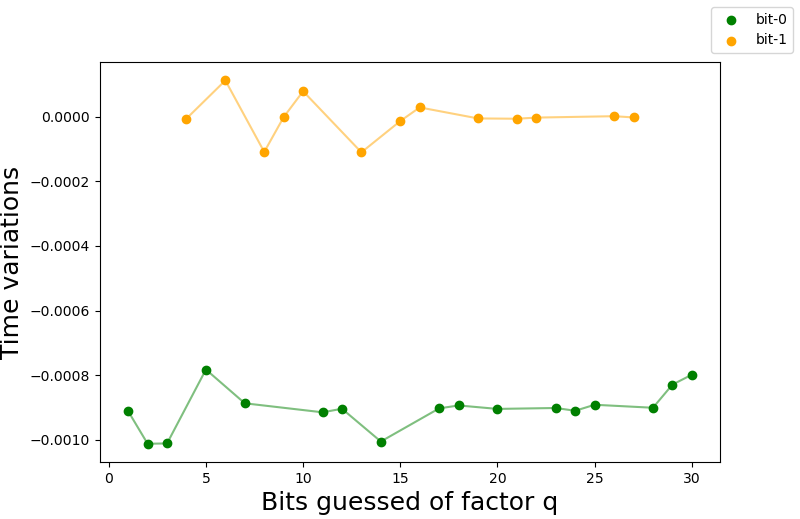
\includegraphics[width=0.65\textwidth]{figures/brumley_and_boneh_output_example}
\end{figure}

During a guess, the attacker queries several times the given device logging elapsed times to perform the attack. But how does the given device simulate the times required by a decryption in an OpenSSL server?
Using the same notation as in \Cref{alg:three}, let $u$ be an integer such that $u =: g \cdot R^{-1} \bmod n$. Now, when the attacker performs a decryption providing $u$ to the device, the latter behaves as follows:
\begin{enumerate}
  \item converts the input $u$ in its Montgomery form (yielding $g$);
  \item initializes elapsed times $t_q := 0$, and $t_p := 0$;
  \item checks if $g < q$, and if true:
    \begin{itemize}
      \item $t_q = t_q + 1000$ (many Montgomery reductions);
      \item $t_q = t_q + 100$ (normal multiplication routine);
    \end{itemize}
  \item[] otherwise ($g \ge self.q$):
    \begin{itemize}
      \item $t_q = t_q + 10$ (few Montgomery reductions);
      \item $t_q = t_q + 10$ (Karatsuba multiplication routine);
    \end{itemize}
  \item repeats step 3. with $p$ (updating $t_p$);
  \item makes the system do nothing for $\frac{\mathcal{N}(t_q + t_p,\ 5)}{1e6}$ seconds.
\end{enumerate}

Magic numbers in step 3. are made up aiming only to follow a consistency in elapsed times.

Another example, that differs from the previous one only by the presence of the blinding technique is the following:

\begin{lstlisting}{backgroundcolor}[language=Python]
    device = Device(num_bits=64, seed=42, blinding=$\textbf{True}$)
    attacker = Attacker(device)
    g = attacker.guess()
    attacker.plot_last_guess()
\end{lstlisting}

\begin{figure}[h]
  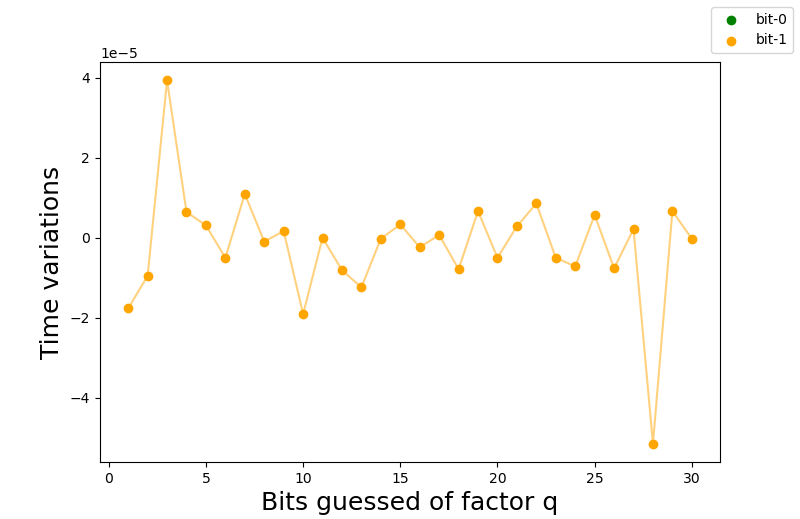
\includegraphics[width=0.65\textwidth]{figures/brumley_and_boneh_output_example_with_blinding}
\end{figure}

Most of the used routines are stored in utilities.py source file. The main functions are dependent on each other, and allow generating RSA factors, generate random prime numbers in a given range, and perform a Miller-Rabin test\cite{bib:boreale}.

%----------------------------------------------------------------------------------------



%----------------------------------------------------------------------------------------
\section{Defences}

As Kocher highlighted in his work, defences like making all operations to take the same amount of time or adding random delays, do not work in practice. The former is hard to implement, especially a platform-independent manner (due to compiler optimizations, cache policies, etc.), and the latter can be sidestepped by increasing the number of samples required for the attack.

Even after almost ten years, Brumley and Boneh stick with the same idea of Kocher, that is that the preferred choice for practical protection against timing attacks should be blinding.

To apply blinding to an RSA system, a random integer $r$, coprime with the public modulus $n$, must be chosen. Now, given a plaintext $m$, its encryption is performed by first multiplying $m$ by $r$, and then computing $(mr)^e \bmod n$, where $\left< n, e \right>$ is the public key of the supposed RSA system. To recover $m$, the resulting ciphertext $c$ must be multiplied by $(r^{-1} \bmod n)^e$, before applying the decryption function.

Blinding was embraced by RSA Security LLC (the American company co-founded by the RSA inventors) in their implementation of RSA, bearing a performance reduction up to 10\% \cite{bib:boreale}.

%----------------------------------------------------------------------------------------



%----------------------------------------------------------------------------------------
\section{Conclusion}

We presented two main timing attacks against RSA, one from Kocher published in 1995, and another from Brumley and Boneh, published in 2005.

First, we introduced some technical background needed to understand how the described attacks work.
Then, we showed Kocher's timing attack: a clear threat to cryptosystems popular in computer security applications when they are based on simple modular exponentiation algorithm.

In addition, we described how Brumley and Boneh made practical an attack to expose RSA private keys on applications based on OpenSSL, a library commonly used in web servers and other SSL application. Their work had a crucial impact on OpenSSL, as well as other crypto libraries, which now implement the defence blinding by default.

%----------------------------------------------------------------------------------------



%----------------------------------------------------------------------------------------
% \section*{References}

\medskip
%\clearpage
{\small
\bibliographystyle{ieee}
\begin{thebibliography}{9}

\bibitem{bib:kocher}{Kocher, P.C., 1996, August. Timing attacks on implementations of Diffie-Hellman, RSA, DSS, and other systems. In Annual International Cryptology Conference (pp. 104-113). Springer, Berlin, Heidelberg.}
\bibitem{bib:openssl}{Brumley, D. and Boneh, D., 2005. Remote timing attacks are practical. Computer Networks, 48(5), pp.701-716.}
\bibitem{bib:boreale}{Boreale, M., 2003. Note per il corso di Sicurezza delle Reti.}
\bibitem{bib:montgomery}{Montgomery, P.L., 1985. Modular multiplication without trial division. Mathematics of computation, 44(170), pp.519-521.}
\bibitem{bib:sliding}{Menezes, A.J., Van Oorschot, P.C. and Vanstone, S.A., 2018. Handbook of applied cryptography. CRC press.}
\bibitem{bib:schindler}{Schindler, W., 2000, August. A timing attack against RSA with the chinese remainder theorem. In International Workshop on Cryptographic Hardware and Embedded Systems (pp. 109-124). Springer, Berlin, Heidelberg.}
\bibitem{bib:coppersmith}{Coppersmith, D., 1997. Small solutions to polynomial equations, and low exponent RSA vulnerabilities. Journal of cryptology, 10(4), pp.233-260.}

\end{thebibliography}
}
%----------------------------------------------------------------------------------------

\end{document}
